\documentclass[10pt,a4paper]{ctexart}
\usepackage[margin=2cm]{geometry}
\usepackage[super]{natbib}
\usepackage{circuitikz}
\usepackage{xcolor}
\usepackage{graphicx}
\usepackage{float}      % 支持 [H] 浮动体选项
\usepackage{hyperref}
\usepackage{amsmath}    % 提供方程环境
\usepackage{physics}    % 简化向量、微分算子语法
\newcommand{\myspace}[1]{\par\vspace{#1\baselineskip}} %自定义空一行
\usepackage{fancyhdr}
\usepackage{makecell}
\usepackage{booktabs} % 用于表格的三线表宏包
\usepackage{tabularx}
\pagestyle{fancy}
\fancyhf{}  % 清除所有页眉页脚
\fancyfoot[C]{\thepage}  % 在页脚中央设置页码
\renewcommand{\headrulewidth}{0pt}  % 去掉页眉横线
\renewcommand{\footrulewidth}{0pt}  % 去掉页脚横线
\newcommand{\thecite}[1]{\textsuperscript{\cite{#1}}}
\usepackage{hyperref}
\usepackage{hyperref}
\hypersetup{
    colorlinks=true,     % 启用颜色链接
    linkcolor=black,     % 内部链接（目录、图表引用等）
    citecolor=black,     % 引用颜色设为黑色
    filecolor=magenta,
    urlcolor=blue,       % 建议URL用蓝色，便于识别
    pdftitle={文档标题},
    pdfpagemode=FullScreen,
}

\usepackage{titlesec}

% 重新定义section格式
\titleformat{\section}
  {\normalfont\Large\bfseries}
  {\chinese{section}、}
  {0pt}
  {}

% 给出常用字号的自定义指令
\newcommand{\chuhao}{\fontsize{42pt}{48pt}\selectfont}
\newcommand{\xiaochu}{\fontsize{36pt}{42pt}\selectfont}
\newcommand{\xiaoer}{\fontsize{18pt}{21.6pt}\selectfont}
\newcommand{\sanhao}{\fontsize{16pt}{20pt}\selectfont}
\newcommand{\xiaosan}{\fontsize{15pt}{18pt}\selectfont}
\newcommand{\sihao}{\fontsize{14pt}{18pt}\selectfont}
\newcommand{\xiaosi}{\fontsize{12pt}{16pt}\selectfont}
\newcommand{\wuhao}{\fontsize{10.5pt}{12.6pt}\selectfont}

% 定义中文数字转换
\titleformat{\section}
  {\normalfont\Large\bfseries}
  {\zhnum{section}、}  % 使用\zhnum而不是\chinese
  {0pt}
  {}

% 标题设置
\title{\xiaochu\textbf{专题研究报告}}
\author{}
\date{}

\begin{document}

\vspace*{36pt} % 顶部空白

% 居中填写区域
\begin{center}
    
\includegraphics[width = 9cm]{figure/head.png}
    
    \xiaochu\textbf{专题研究报告}
    % 预留空白区域
    \vspace{13pt}
    \vspace{13pt}
    \vspace{13pt}
    \vspace{13pt}
    
    \sanhao\textbf{标题：\underline{\makebox[10cm]{心电采集系统中前置滤波电路的设计 }}} \\[10pt]
    
    % 预留空白区域
    \myspace{6}
    
   \sihao\textbf{班级：\underline{\makebox[6cm]{}}} \\[10pt]
    \sihao\textbf{姓名：\underline{\makebox[6cm]{}}} \\[10pt]
    \sihao\textbf{学号：\underline{\makebox[6cm]{}}} \\[30pt]
    
    
    \vspace{18pt}
    
\end{center}

\newpage

\section{研究背景与意义}
心电信号是人类最早研究并应用于临床的生物电信号之一，自1903年心电图发明以来，其在生物医学与工程学领域的记录、处理与诊断技术均得到了飞速发展\cite{key1, key2}。
心电信号反映了心脏的电活动状态，对于心脏疾病的诊断与治疗具有重要意义。心电信号采集与处理系统是现代心脏病诊断、监护和研究的基石。

然而，心电信号通常伴随着各种噪声和干扰，如工频干扰、肌电干扰等，这些噪声会严重影响心电信号的质量和诊断的准确性。因此，设计高效的前置滤波电路对于提高心电信号的质量具有重要作用。
 


\myspace{2}
\section{系统要求与设计指标}
心电信号幅值范围一般是0.5mV到5mV，频率范围约为0.05Hz到100Hz，但是超过90\%能量集中在0.25Hz到30Hz之间\cite{signal_char}。

由于心电信号非常微弱，所以要求滤波电路增益较高，一般在100倍以上,输入阻抗高，减少分压损失。由于是带通滤波器，可以考虑使低通滤波器和高通滤波器分别具有10倍左右的增益，构成带通滤波器。

根据心电信号的频率特性，滤波电路带宽应覆盖0.05Hz到100Hz.

滤波电路还应具有低噪声、低功耗等特性，考虑到本课程所学暂时忽略这些要求，重点放在滤波特性和增益设计上。



\section{设计思路与方法}
\subsection{滤波器类型选择}
主流的滤波器类型包括有源滤波器和无源滤波器两大类。无源滤波器由电阻、电容和电感等无源元件组成，结构简单，但无法提供增益，且受限于元件参数，难以实现高性能滤波。
而有源滤波器则利用运算放大器等有源元件，可以实现高增益、低噪声和良好的频率响应特性。因此，本设计选择有源滤波器作为前置滤波电路的核心。

有源滤波器中巴特沃斯滤波器、切比雪夫滤波器和贝塞尔滤波器是常见的类型。
它们的特性对比如下表所示\cite{filter_design}：

\begin{table}[H]
\centering
\caption{滤波器近似法类型比较表}
\label{tab:filter_comparison}
\begin{tabularx}{\textwidth}{XcXX}
\toprule
\textbf{滤波器类型} & \textbf{带通} & \textbf{过渡区域} & \textbf{阶跃响应} \\
\midrule
巴特沃兹滤波器 & 带通中最大的平坦幅度 & 比贝塞尔滤波器陡峭，但不如切比雪夫性能好 & 有一些过冲和振铃，但低于切比雪夫滤波器 \\
\hline
切比雪夫滤波器 & 带通中的纹波 & 比巴特沃兹滤波器和贝塞尔滤波器陡峭 & 过冲和振铃合理 \\
\hline
贝塞尔滤波器 & 带通中的平坦幅度响应 & 比巴特沃兹滤波器和切比雪夫滤波器慢 & 与巴特沃兹滤波器和切比雪夫滤波器相比，过冲或振铃非常小 \\
\bottomrule
\end{tabularx}
\end{table}

切比雪夫滤波器带通特性具有纹波，即使是很小的波纹（如0.5dB），也会导致信号不同频率分量被放大倍数不一致，相当于引入了频率失真。这对于需要保真度的生物信号来说是不可取的，对于后续利用心电信号分析人体医学信息造成很大干扰，甚至于误诊，不宜采用。
此外，切比雪夫滤波器的时域响应有明显的过冲与振铃现象，也不适合心电信号的处理,可能会在陡峭的QRS波后产生虚假的振荡波形，容易被误读为病理特征。

贝塞尔滤波器的频率响应虽然平坦，但过渡区域较宽，滤波器阶数需要较高才能达到所需的截止特性，增加了电路复杂度和成本。考虑到心电采集设备对成本和复杂度的要求，贝塞尔滤波器也不太适合。

巴特沃斯滤波器具有平坦的通带响应，适合心电信号的频率特性，虽然时域响应有一定的过冲和振铃，但低于切比雪夫滤波器，可以接受，因此本设计选择巴特沃斯滤波器作为滤波器类型。

阶数越高，滤波器的频率响应越陡峭，但电路复杂度和成本也随之增加。考虑到心电信号的频率特性和实际应用需求，本设计选择二阶巴特沃斯滤波器作为前置滤波电路的核心。

综上所述，选择二阶有源巴特沃斯滤波器作为心电采集系统前置滤波电路的核心。通过高通滤波器与低通滤波器的级联实现带通滤波功能，同时满足心电信号的频率特性和增益要求。
\subsection{滤波器设计}
在考虑增益不为1的情况下，二阶低通巴特沃斯滤波器的传递函数为：
\begin{equation}
H_{LP}(s) = \frac{A \omega_0^2}{s^2 + \sqrt{2} \omega_0 s + \omega_0^2}
\end{equation}
其中，$A$为增益，$\omega_0$为截止角频率。

根据心电信号的频率特性，设计低通滤波器的截止频率$f_c$为100Hz，对应的截止角频率$\omega_0 = 2 \pi f_c = 200 \pi$ rad/s。

二阶高通巴特沃斯滤波器的传递函数为：
\begin{equation}
H_{HP}(s) = \frac{A s^2}{s^2 + \sqrt{2} \omega_0 s + \omega_0^2}
\end{equation}
设计高通滤波器的截止频率$f_c$为0.05Hz，对应的截止角频率$\omega_0 = 2 \pi f_c = 0.1 \pi$ rad/s，增益$A$同样设为10。
\myspace{2}

\section{低通滤波器电路设计与仿真}
\subsection{电路设计}
根据二阶低通巴特沃斯滤波器的传递函数，选择Sallen-Key结构实现。设定增益$A=10$，截止频率$f_c=100Hz$。 电路拓扑结构如图\ref{fig:LF_circuit}所示。
\begin{figure}[H]
    \centering
    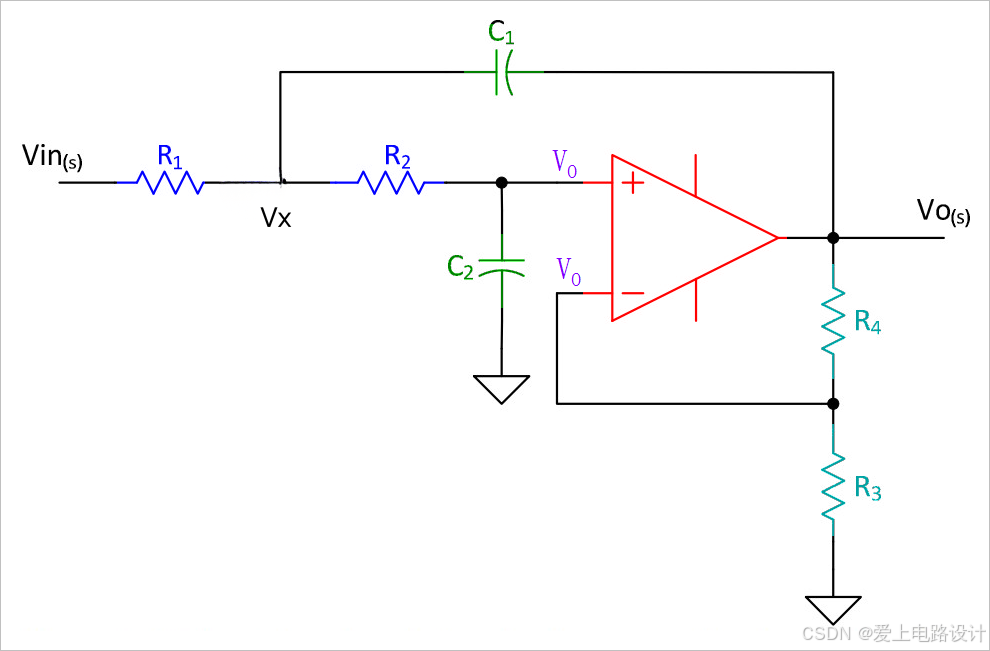
\includegraphics[width=0.4\textwidth, height=0.2\textheight]{figure/LF_circuit.png}
    \caption{低通滤波器电路拓扑结构}
    \label{fig:LF_circuit}
\end{figure}
根据电路方程组：
\begin{equation}
\begin{cases}
\frac{V_{in}-V_x}{R_1}=\frac{V_x-V_0}{R_2}+sC_1(V_x-V_{out}) \\
V_{0}=\frac{R_3}{R_3 + R_4} V_{out} \\
V_{0} = \frac{1}{1+sC_2R_2} V_x \\
\end{cases}
\end{equation}
计算电路传递函数\cite{tf}：
\begin{equation}
H(s) =  \frac{K}{R_1 R_2 C_1 C_2 s^2 + [R_1 C_2 + R_2 C_2 - (K-1)R_1 C_1]s + 1}
\end{equation}
有
\begin{equation}
  \begin{cases}
    K = 1 + \frac{R_4}{R_3} \\
    \omega_0^2 = \frac{1}{R_1 R_2 C_1 C_2} \\
    \frac{\sqrt{2}}{\omega_0}  =R_1 C_2 + R_2 C_2 - (K-1)R_1 C_1
  \end{cases}
\end{equation}
接下来确定元件参数。 
首先确定增益$K=10$，考虑到希望滤波器输出电阻较小，故选择$R_3 = 10\Omega$，$R_4 = 90\Omega$。

接下来令$C_1=C_2=C$,$R_2=R, R_1=mR$。
则有(将(5)式中后两个方程消去$\omega_0^2$得到)：
\begin{equation}
  1+m(2-K)= \sqrt{2m}
\end{equation}
由此计算出$m \approx 0.205$，即$R_1 \approx 0.205 R_2$。

根据截止频率$f_c=100Hz$，计算出：
\begin{equation}
RC = \frac{1}{2 \pi f_c \sqrt{m}} \approx 3.515 \times 10^{-3} s
\end{equation}
结合标称值，希望输入电阻较大，因此选择小电容$C=1 nF$,$R_2=3.6 M\omega, R_1=750 k\omega$.
\subsection{仿真结果}
使用LTspice对设计的低通滤波器电路进行仿真，测量电路的中频增益、截止频率、输入电阻与输出电阻。

仿真结果显示，中频增益约$A_m=20.1 dB$，截止频率约$f_c=114.41Hz$,输入电阻$R_{in}$在0.05Hz-100Hz范围内随频率增大先减小后几乎不变，变化范围大约是$229 k\Omega$到$390.5 M\Omega$，符合设计指标。
输出电阻$R_{out}$也随频率先几乎不变再减小，变化范围大约是$1.8 \Omega$-$6.2 \Omega$。

可以看到仿真结果与设计指标较为接近，满足心电信号采集系统的需求。

电路仿真结果如下。
\begin{figure}[H]
    \centering
    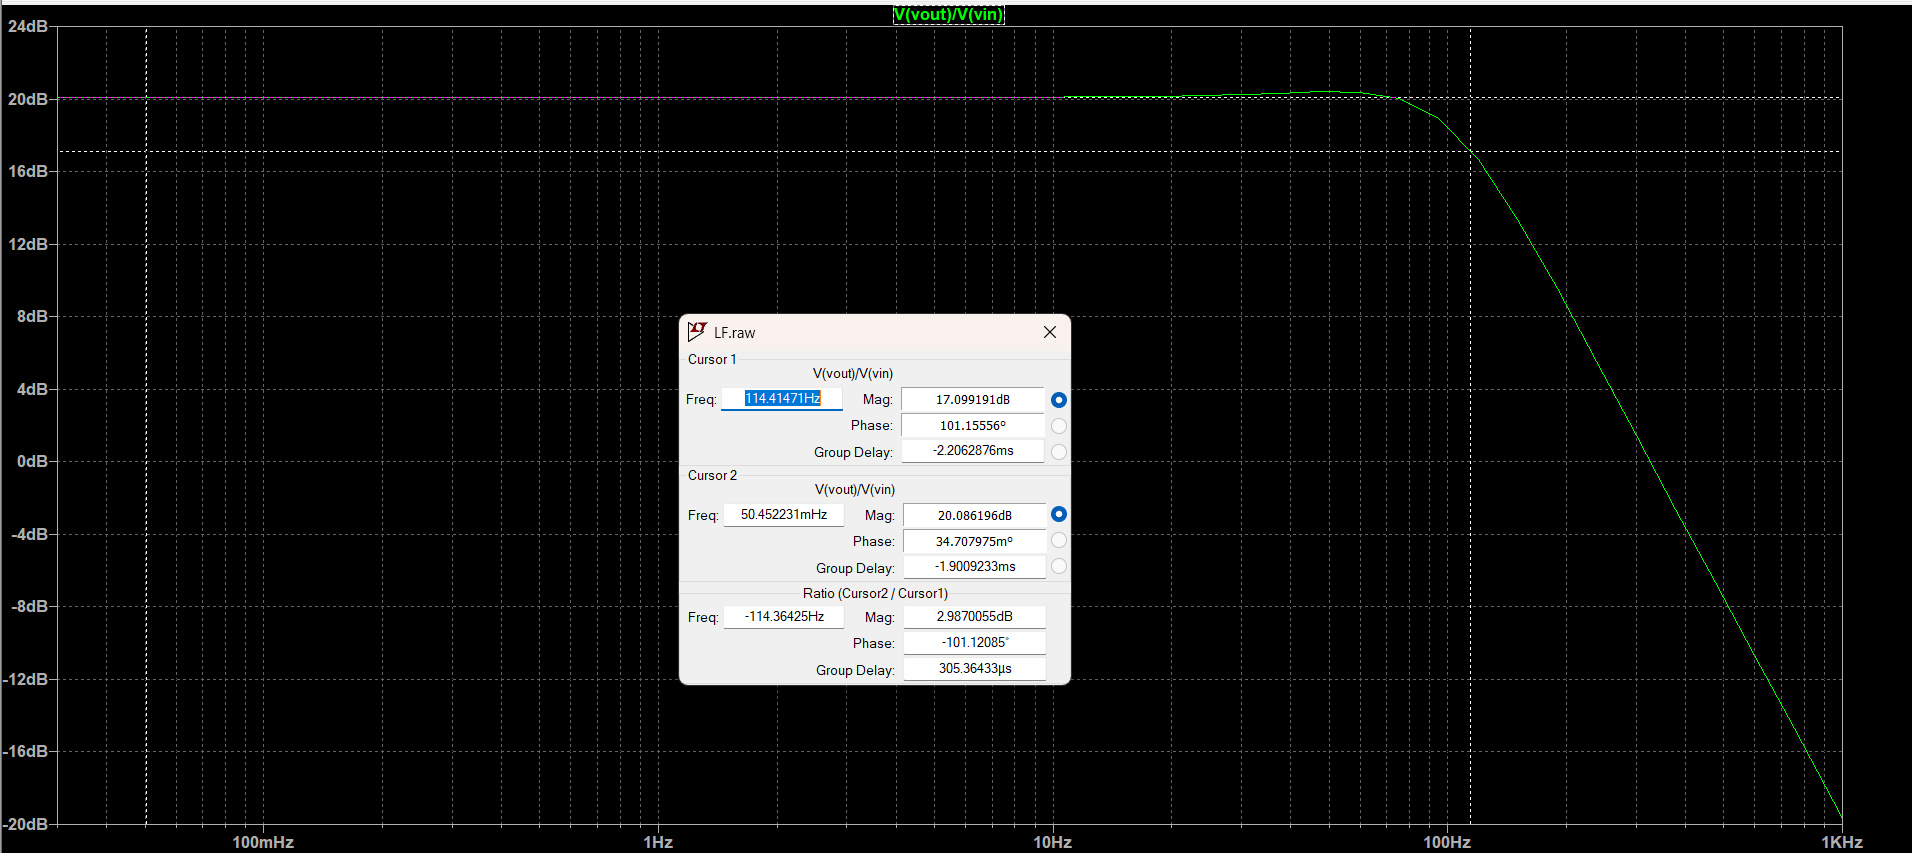
\includegraphics[width=0.4\textwidth, height=0.2\textheight]{figure/LF_sti/LF_A.png}
    \caption{低通滤波器增益频率特性曲线}
    \label{fig:LF_A}
\end{figure}
\begin{figure}[H]
    \centering
    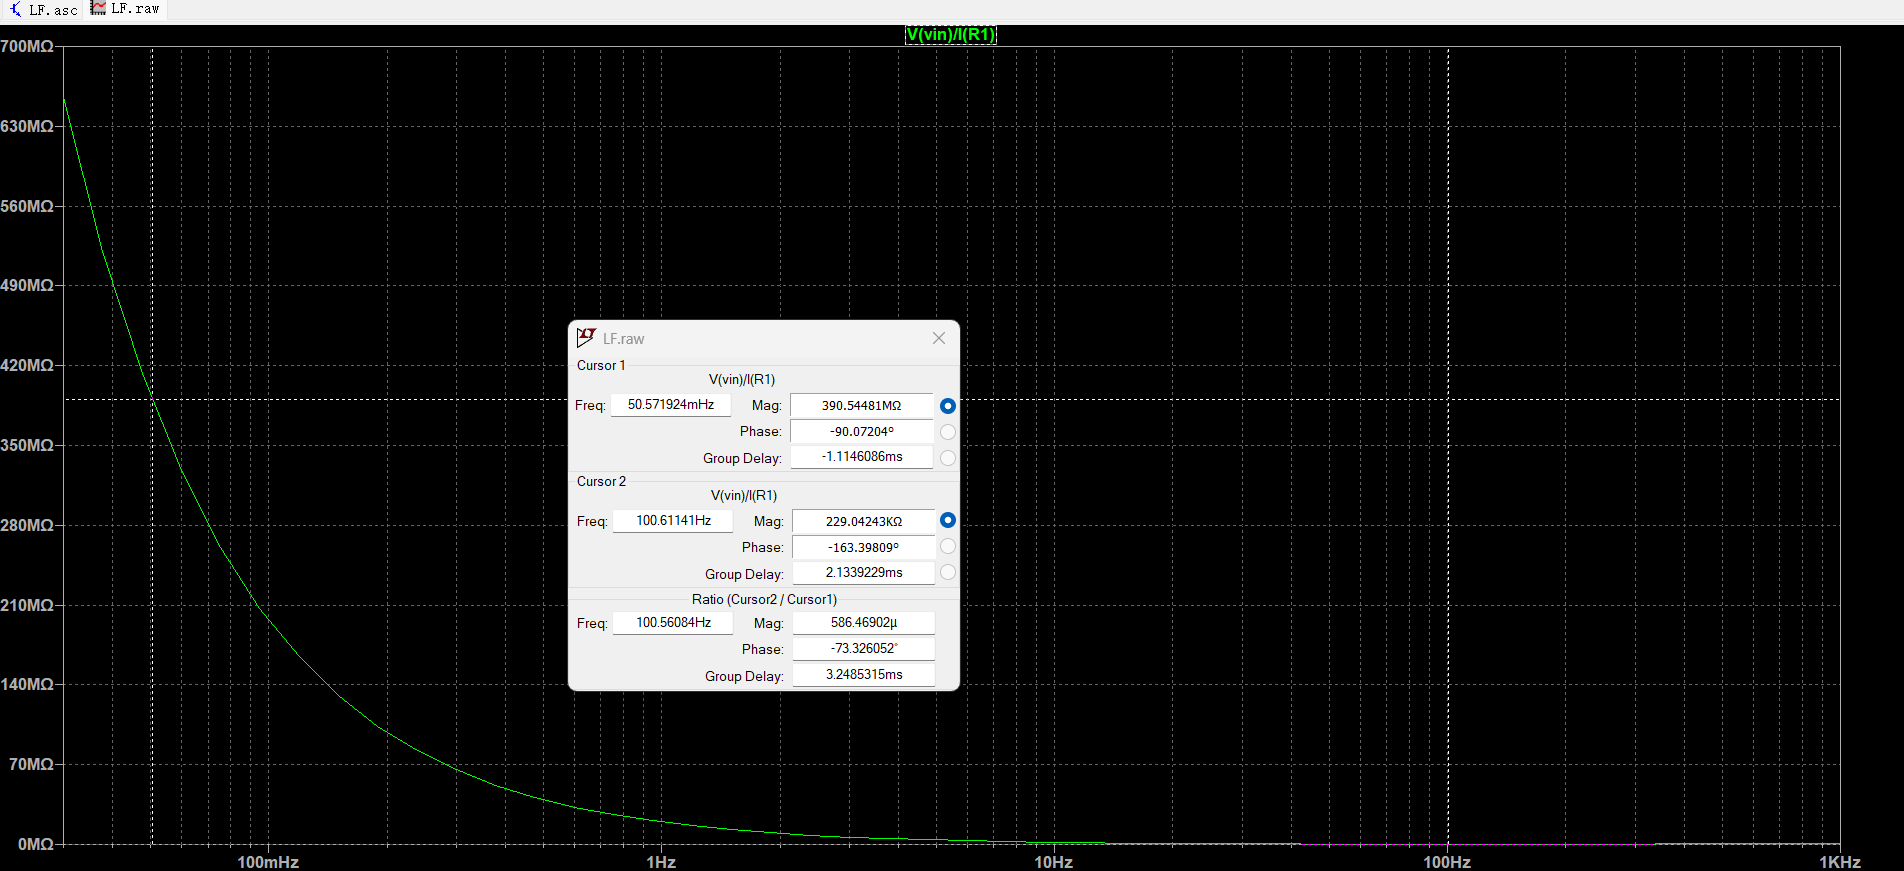
\includegraphics[width=0.4\textwidth, height=0.2\textheight]{figure/LF_sti/LF_ri.png}
    \caption{低通滤波器输入电阻频率特性曲线}
    \label{fig:LF_ri}
\end{figure}
\begin{figure}[H]
    \centering
    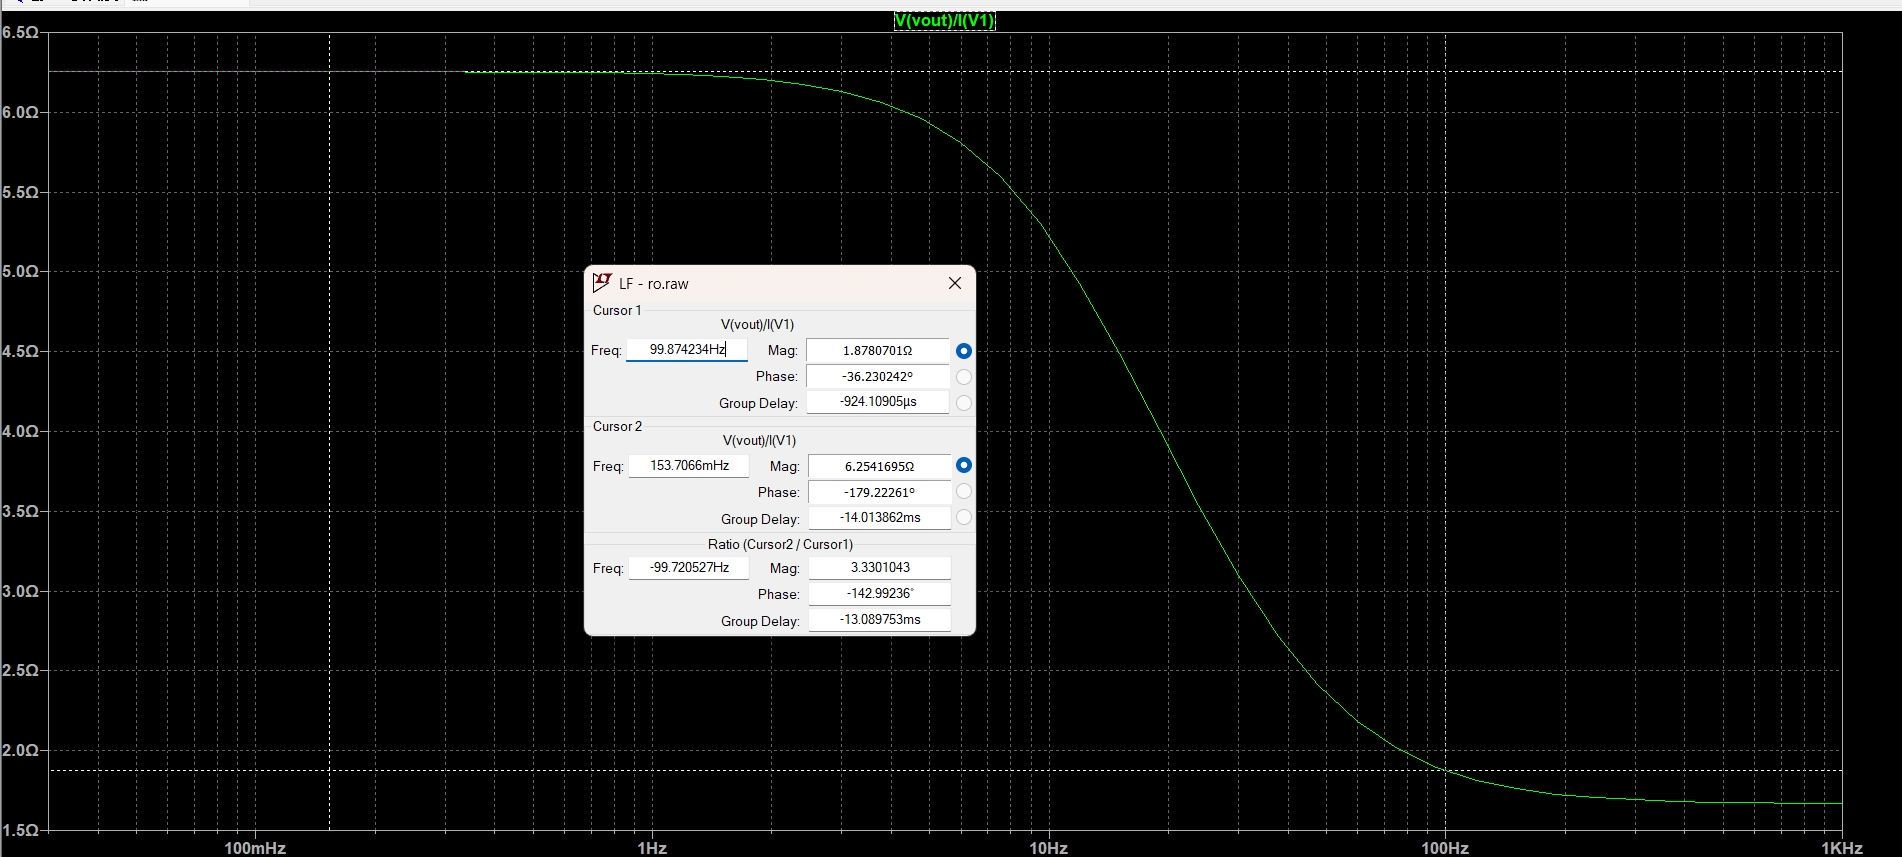
\includegraphics[width=0.4\textwidth, height=0.2\textheight]{figure/LF_sti/LF_ro.png}
    \caption{低通滤波器输出电阻频率特性曲线}
    \label{fig:LF_ro}
\end{figure}
\section{高通滤波器电路设计与仿真}
\subsection{电路设计}
根据二阶高通巴特沃斯滤波器的传递函数，选择Sallen-Key结构实现。设定增益$A=10$，截止频率$f_c=0.05Hz$。 电路拓扑结构如图\ref{fig:HF_circuit}所示。
\begin{figure}[H]
    \centering
    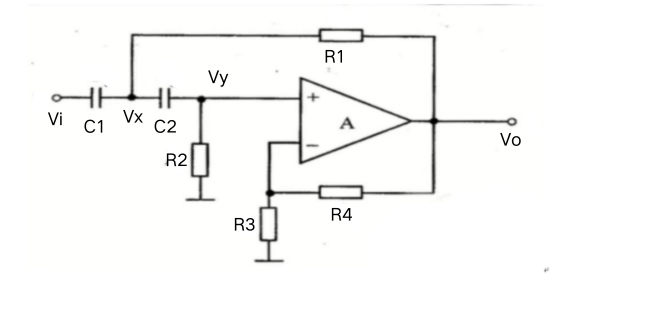
\includegraphics[width=0.4\textwidth, height=0.2\textheight]{figure/HF_circuit.png}
    \caption{高通滤波器电路拓扑结构}
    \label{fig:HF_circuit}
\end{figure}
根据电路方程组：
\begin{equation}
\begin{cases}
sC_1(V_{i}-V_x)=sC_2 (V_x-V_y) + \frac{V_x - V_o}{R_1} \\
V_{y}=\frac{R_3}{R_3 + R_4} V_{o} \\
V_{y} = \frac{sC_2R_2}{(1 + sC_2 R_2)} V_x \\
\end{cases}
\end{equation}
计算电路传递函数：
\begin{equation}
H(s) =  \frac{K R_1 R_2 C_1 C_2 s^2}{R_1 R_2 C_1 C_2 s^2 + [R_1 C_1 + R_1 C_2 - (K-1)R_2 C_2]s + 1}
\end{equation}
因此有
\begin{equation}
  \begin{cases}
    K = 1 + \frac{R_4}{R_3} \\
    \omega_0^2 = \frac{1}{R_1 R_2 C_1 C_2} \\
    \frac{\sqrt{2}}{\omega_0}  =R_1 C_1 + R_1 C_2 - (K-1)R_2 C_2
  \end{cases}
\end{equation}
和低通滤波器一样，考虑到希望滤波器输出电阻较小，故选择$R_3 = 10\Omega$，$R_4 = 91\Omega$，增益$K=10$。

接下来令$C_1=C_2=C$,$R_2=R, R_1=mR$。
则有(将(10)式中后两个方程消去$\omega_0
^2$得到)：
\begin{equation}
  2m+1-K= \sqrt{2m}
\end{equation}
由此计算出$m \approx 3.23$，即$R_1 \approx 3.23 R_2$。
根据截止频率$f_c=0.05Hz$，计算出：
\begin{equation}
RC = \frac{1}{2 \pi f_c \sqrt{m}} \approx 1.77 s
\end{equation}
考虑到输入电阻与C的关系，尽量使C较小，因此选择$C=1 \mu F$,$R_2=1.8 M\Omega, R_1=6.2 M\Omega$.

\subsection{仿真结果}

使用LTspice对设计的高通滤波器电路进行仿真，测量电路的中频增益、截止频率、输入电阻与输出电阻。
仿真结果显示，中频增益$A_m=20.1 dB$，截止频率$f_c=0.041Hz$,输入电阻$R_{in}$在0.05Hz-100Hz范围内随频率增大先减小再几乎不变，变化范围大约是$1.1 M\Omega$到$1.2 M\Omega$，符合设计指标。
输出电阻$R_{out}$随频率增大而先增大后基本不变，变化范围大约是$6 \Omega$-$30\Omega$。

仿真结果如下图所示
\begin{figure}[H]
    \centering
    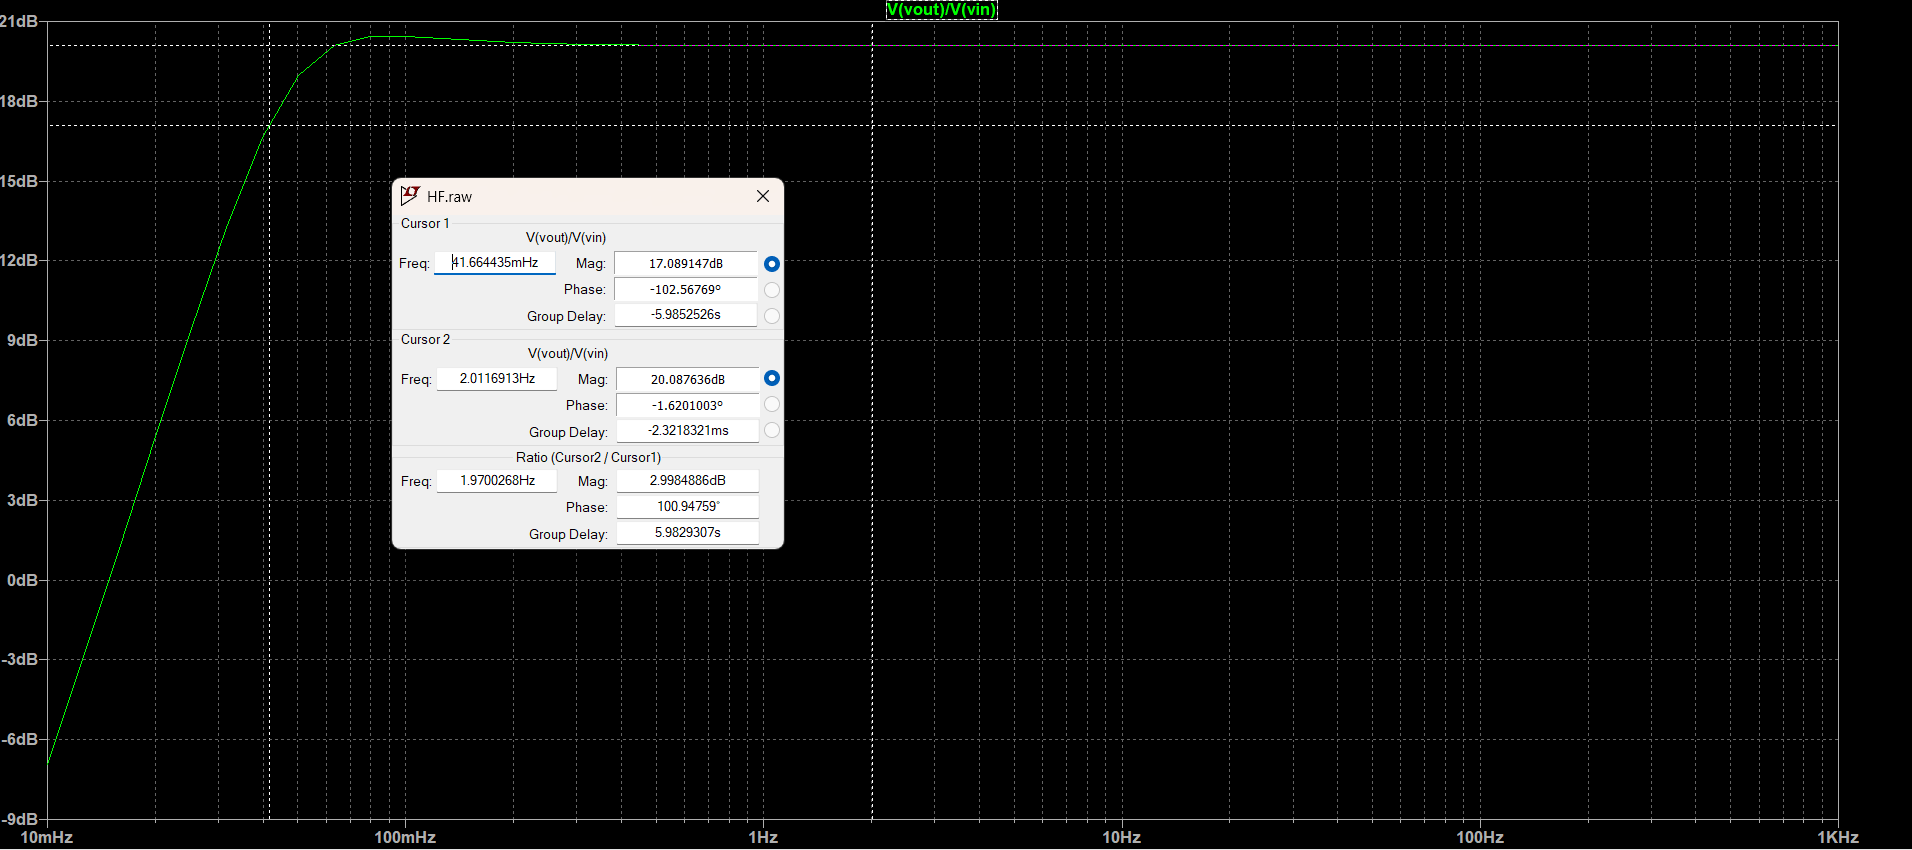
\includegraphics[width=0.4\textwidth, height=0.2\textheight]{figure/HF_sti/HF_A.png}
    \caption{高通滤波器增益频率特性曲线}
    \label{fig:HF_A}
\end{figure}

\begin{figure}[H]
    \centering
    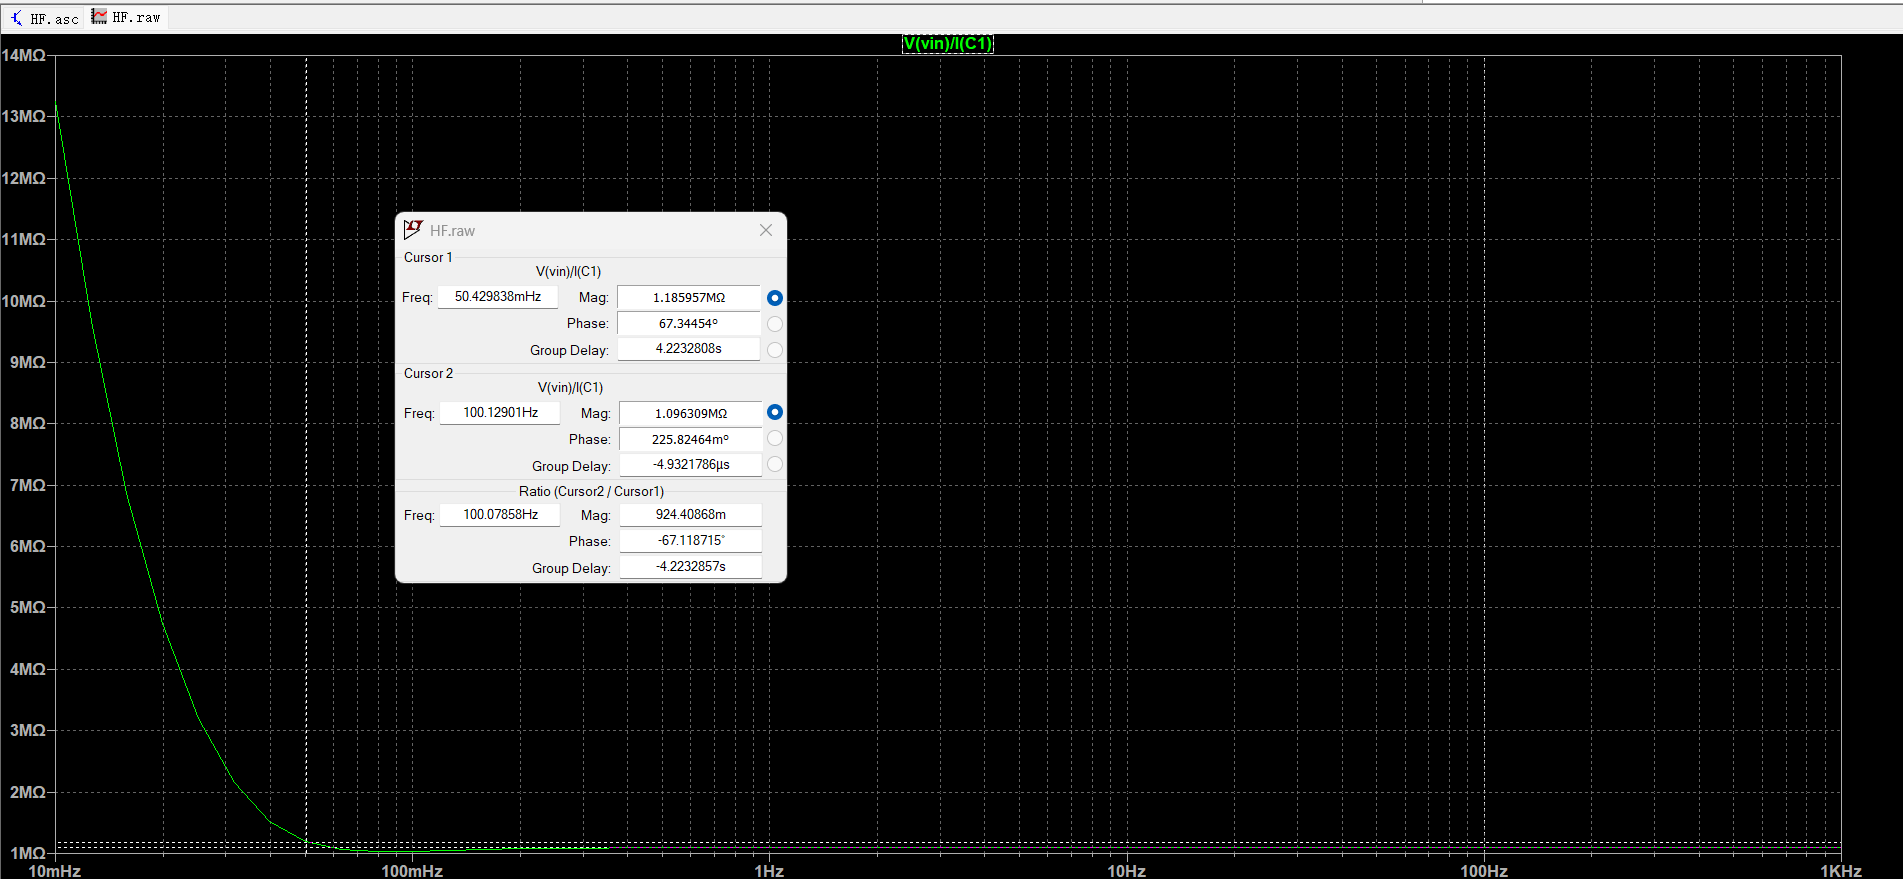
\includegraphics[width=0.4\textwidth, height=0.2\textheight]{figure/HF_sti/HF_ri.png}
    \caption{高通滤波器输入电阻频率特性曲线}
    \label{fig:HF_ri} 
\end{figure}

\begin{figure}[H]
    \centering
    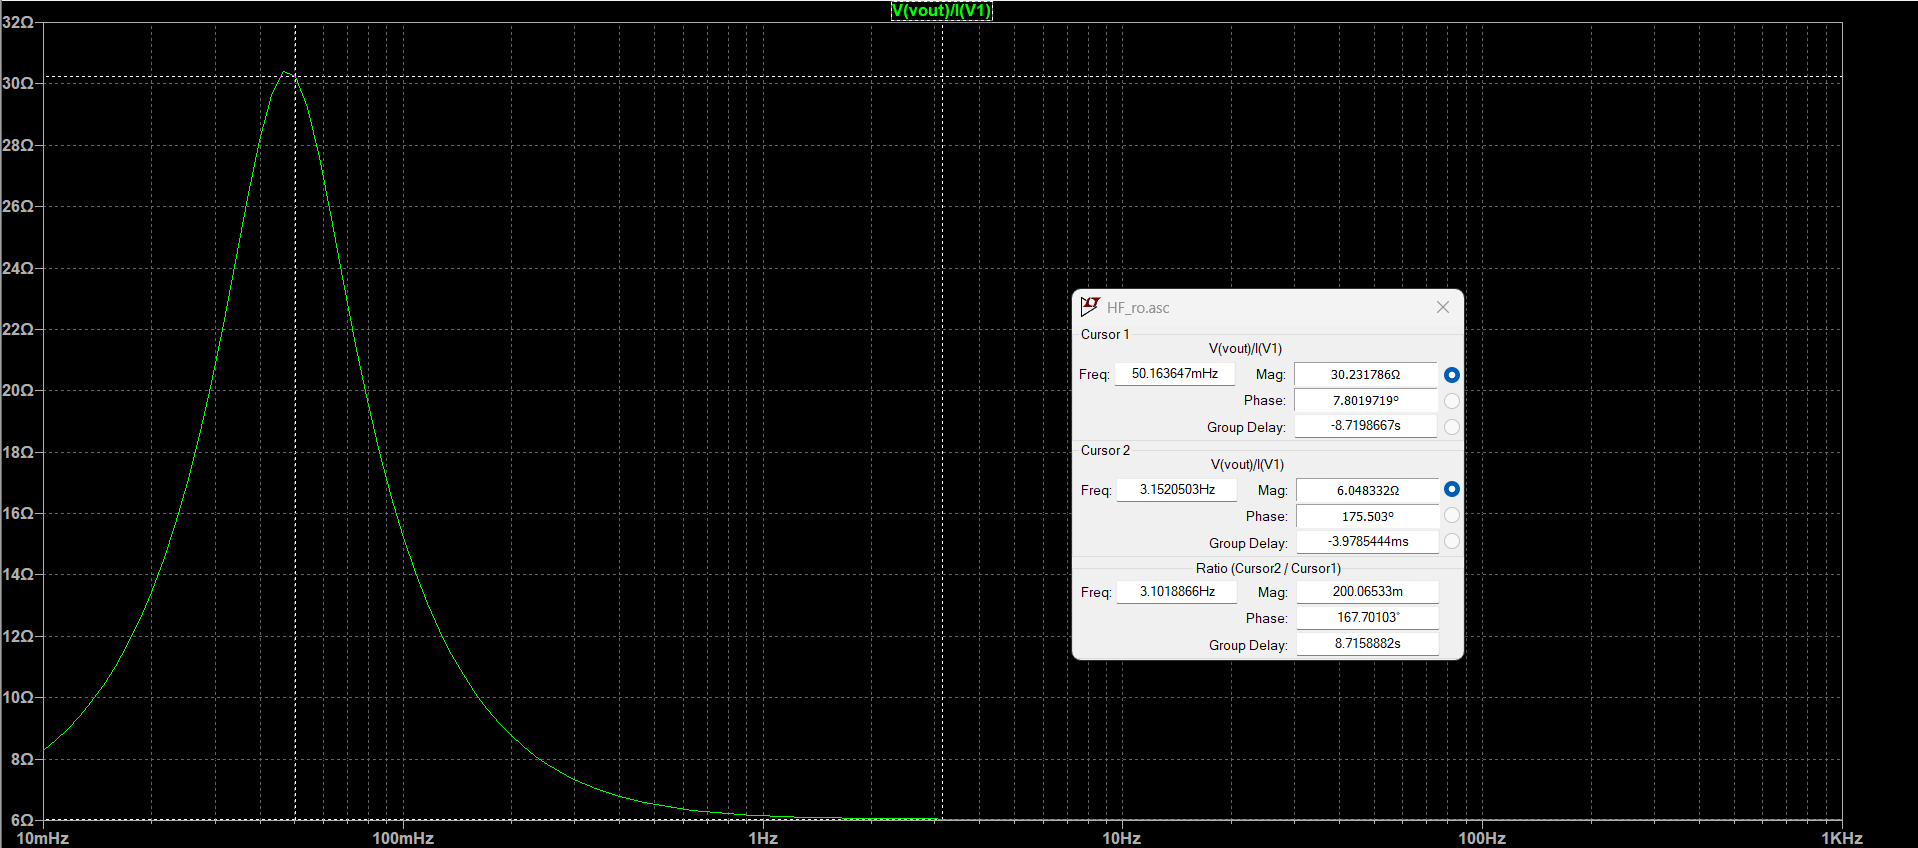
\includegraphics[width=0.4\textwidth, height=0.2\textheight]{figure/HF_sti/HF_ro.png}
    \caption{高通滤波器输出电阻频率特性曲线}
    \label{fig:HF_ro}
\end{figure}

\section{级联电路仿真}
将高通滤波器接在低通滤波器之前，构成带通滤波器，对整体电路进行仿真，测量整体增益、截止频率、输入输出阻抗。
仿真结果显示，整体电路中频增益约为40dB，截止频率约为41mHz与116Hz，输入输出阻抗均满足设计要求，符合心电信号采集系统的需求。
输入阻抗与高通滤波器的输入阻抗相近随频率增大先减小再几乎不变（有小段增加），变化范围约$1.1M \Omega$-$1.2M \Omega$，输出阻抗随频率增大，先保持平坦，之后逐渐增大，从约$6 \Omega$增大到$20 \Omega$。波形没有和低通滤波器保持一致，是受到了高通滤波器的阻抗影响，但是仍符合设计要求。
仿真结果如下图所示
\begin{figure}[H]
    \centering
    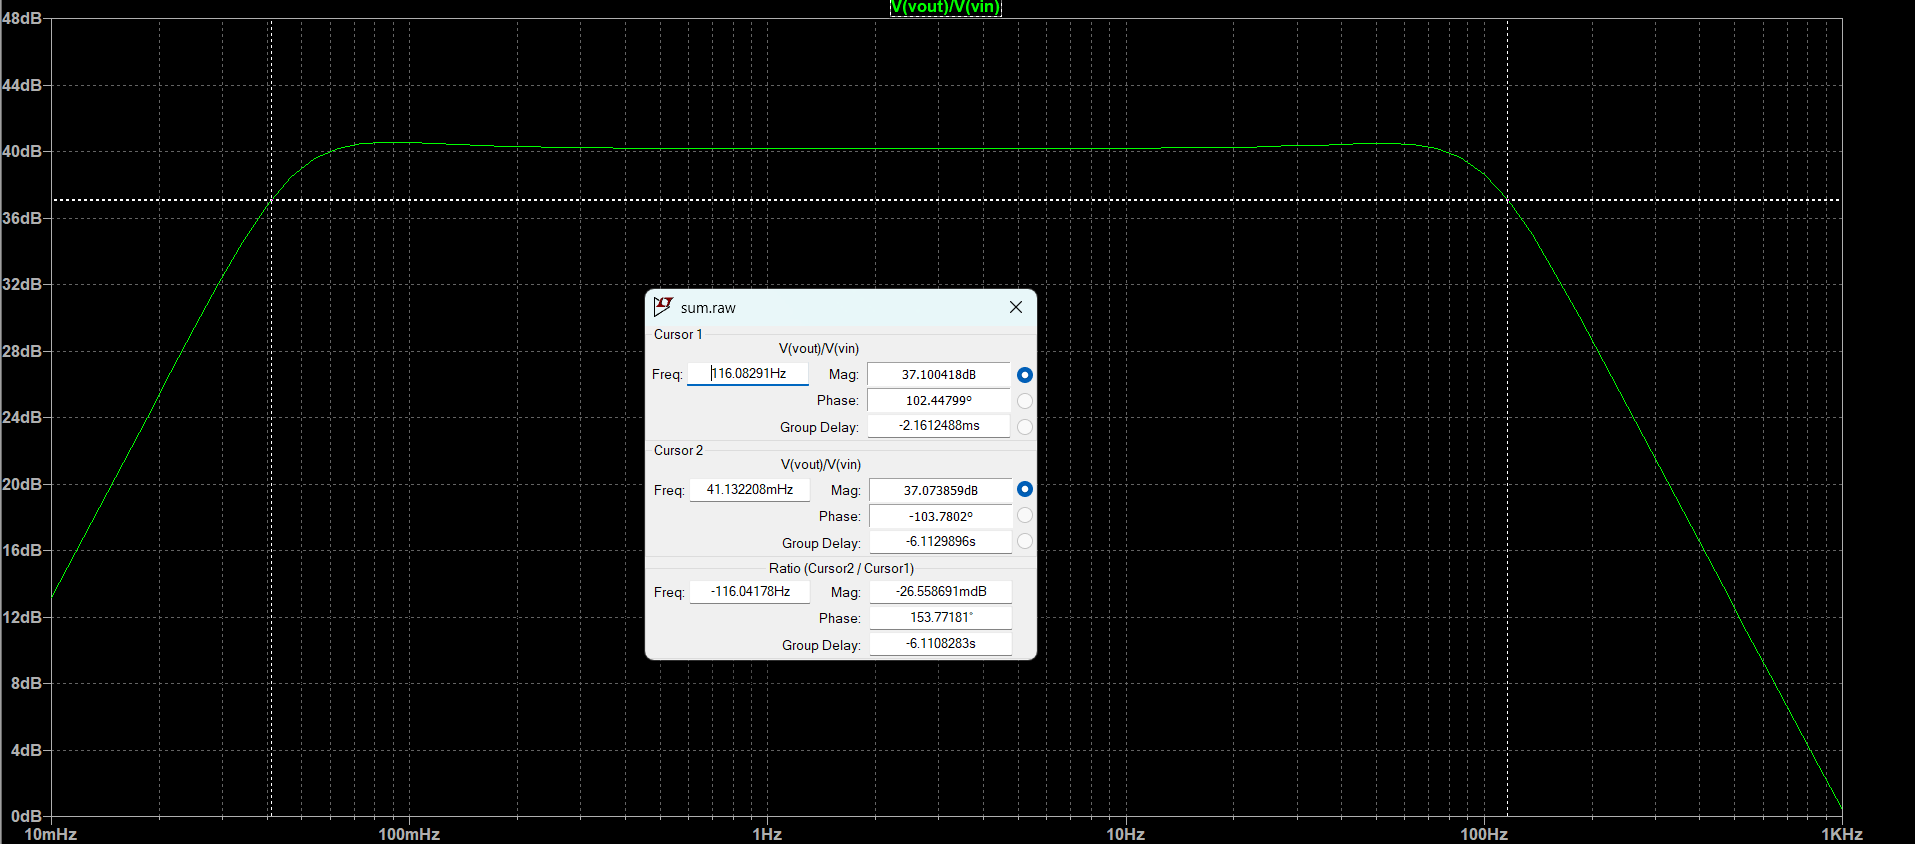
\includegraphics[width=0.4\textwidth, height=0.2\textheight]{figure/sum_sti/sum_A.png}
    \caption{带通滤波器增益频率特性曲线}
    \label{fig:sum_A}
\end{figure}
\begin{figure}[H]
    \centering
    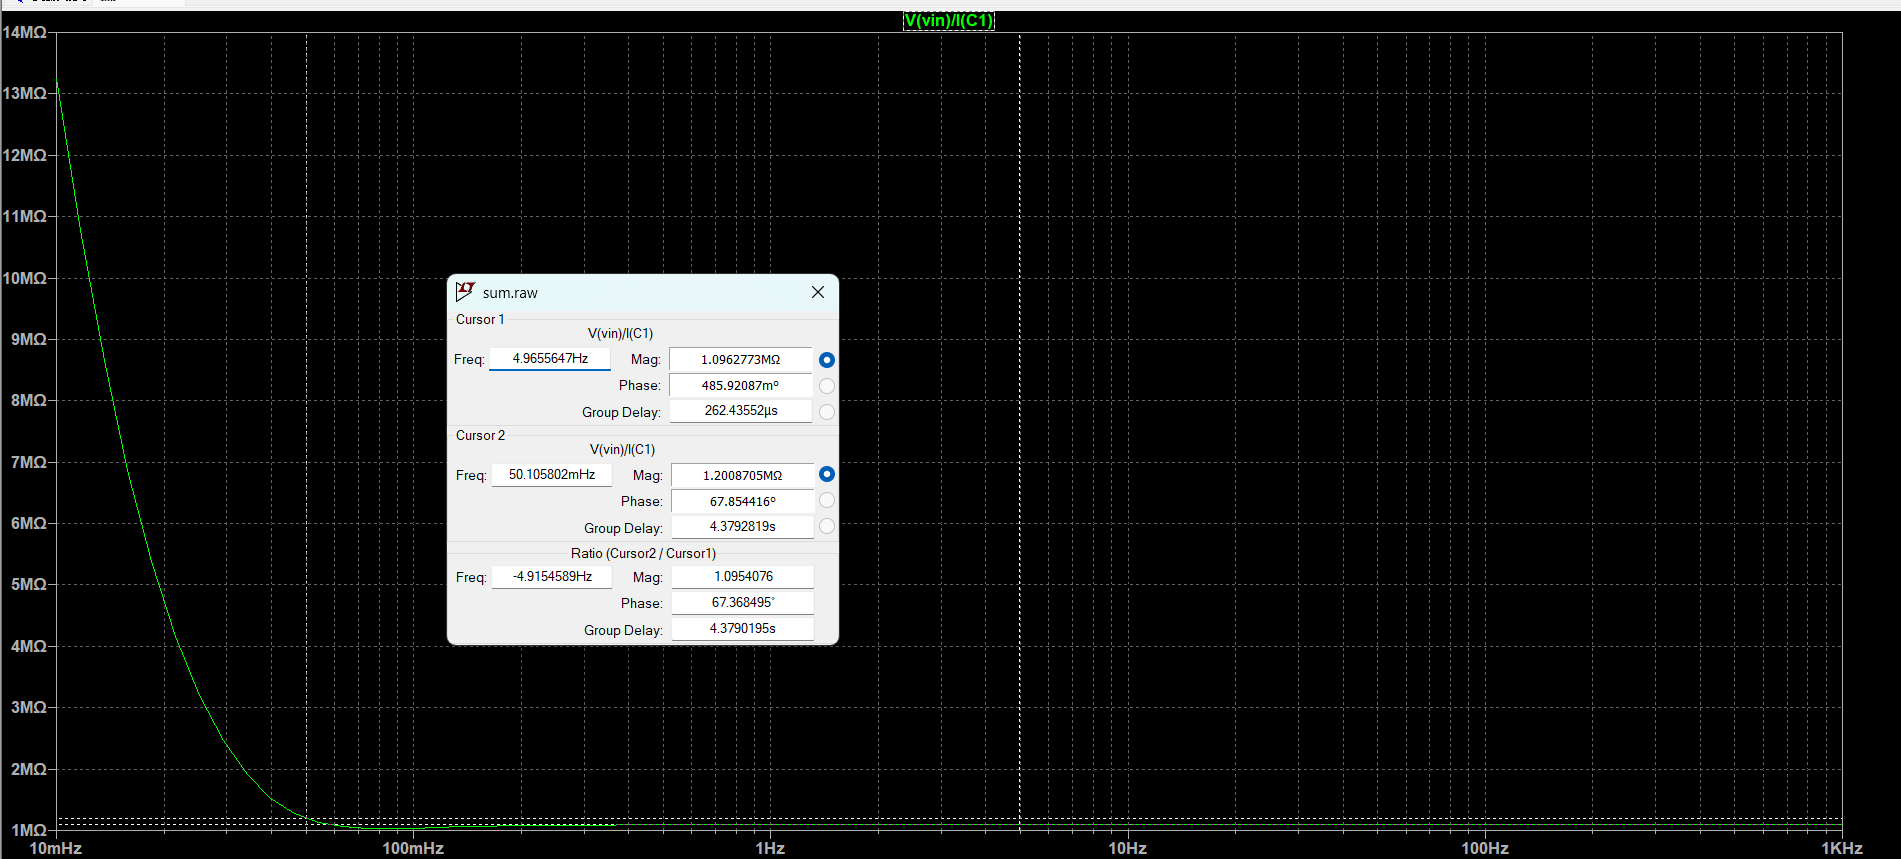
\includegraphics[width=0.4\textwidth, height=0.2\textheight]{figure/sum_sti/sum_ri.png}
    \caption{带通滤波器输入电阻频率特性曲线}
    \label{fig:sum_ri}
\end{figure}
\begin{figure}[H]
    \centering
    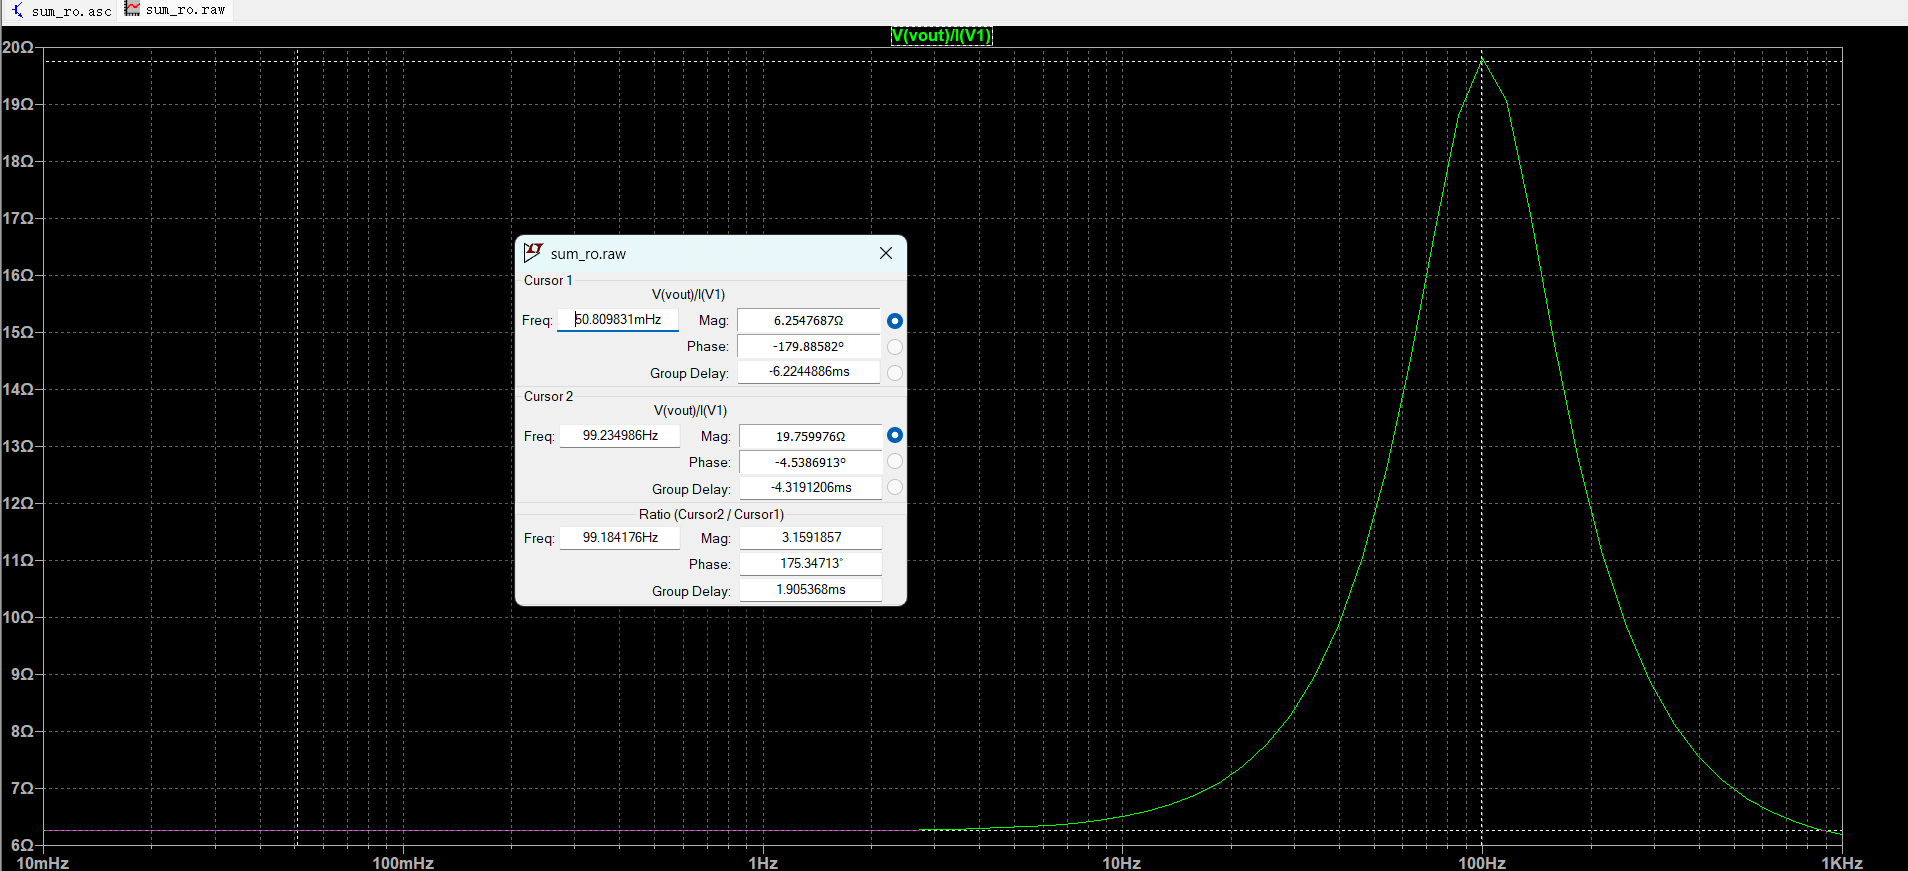
\includegraphics[width=0.4\textwidth, height=0.2\textheight]{figure/sum_sti/sum_ro.png}
    \caption{带通滤波器输出电阻频率特性曲线}
    \label{fig:sum_ro}
\end{figure}
\section{结论}

本报告完成了心电采集系统前置滤波电路的设计与仿真。通过对心电信号特点的分析，确定了带通范围0.05-100Hz、高增益的设计要求。


经比较三种滤波器类型，选择二阶巴特沃斯滤波器，因其通带平坦，能较好地保持心电信号形态。采用Sallen-Key结构分别设计了截止频率为0.05Hz的高通滤波器和100Hz的低通滤波器，每级增益设为10倍。

仿真结果表明：

高通滤波器截止频率0.041Hz，增益20.1dB

低通滤波器截止频率114.41Hz，增益20.1dB

两级级联可获得约40dB总增益

输入输出阻抗满足要求

本设计验证了利用课程所学运算放大器、频率响应等知识，能够构建符合心电信号采集基本要求的滤波电路。虽然实际应用还需考虑更多因素，但本报告为生物电信号处理提供了基础的设计思路和方法。
\begin{thebibliography}{99} 
    \bibitem{key1} Einthoven, W. (1903). The galvanometric registration of the human electrocardiogram, along with a judgment of the application of capillar-electrometer in the physiology. Pflügers Archiv für Die Gesamte Physiologie Des Menschen Und Der Tiere, 99(9/10), 472-480.
    \bibitem{key2} Martinek, R., Ladrova, M., Sidikova, M., Jaros, R., Behbehani, K., Kahankova, R., \& Kawala-Sterniuk, A. (2021). Advanced bioelectrical signal processing methods: Past, present and future Approach—Part I: Cardiac signals. Sensors (Basel, Switzerland), 21(15), 5186. https://doi.org/10.3390/s21155186
    \bibitem{signal_char}赵泰.(2011).便携式心电信号采集系统设计(硕士学位论文,重庆大学).硕士\url{https://kns.cnki.net/kcms2/article/abstract?v=hyKDWyHWvTuIf6RDTycEBP8LxE69_9Ks0PNm6N7_JnpbG-r6mLcfcWlzRUmKG-FL6uDeTaKH2XXVLtcLCIlkSyIXIggiypVAvElNuppZJ4ug60xgrHM6rRu1b4TqRD9oPzmNpf_OnFQHyyE7iuf00kzeav7U9NFkXbu8nfr9qgqjceDpbWxXQA==&uniplatform=NZKPT&language=CHS}
    \bibitem{filter_design} Baker, B. (2014). 有源模拟滤波器的快速设计. 电源世界, (4), 39-41.
    \bibitem{tf}Texas Instruments. (2022, August). *Design of anti-aliasing filters for single-supply ADCs* (Publication No. ZHCAc38D) [Application report]. Retrieved from https://www.ti.com.cn/cn/lit/an/zhcac38d/zhcac38d.pdf
\end{thebibliography}



\vspace{1cm}

\end{document}